\documentclass[cn, 11pt, chinese, show]{elegantbook}
\usepackage{fontspec}
\usepackage{xeCJK}
% \setCJKmainfont{SourceHanSerifCN-Regular}
% \setmainfont{texgyrepagella-regular.otf}
\setmonofont{Hack-Regular}

\title{数学建模竞赛信息管理软件——使用文档}
\subtitle{华北理工大学数学建模协会}

\author{16计科兰铃}
\date{May 10, 2020}
\version{2.0}
\bioinfo{依赖}{Elegant\LaTeX{} Program}

\extrainfo{沿着旧地图,找不到新大陆}

\logo{logo-blue.png}
\cover{cover.jpg}

% 本文档命令
\usepackage{array}
\newcommand{\ccr}[1]{\makecell{{\color{#1}\rule{1cm}{1cm}}}}


\begin{document}

\maketitle
\frontmatter

\chapter*{特别声明}
\markboth{Introduction}{前言}

这个软件被开发的原因是整理建模协会历年参赛人员的信息。在过去的 2019 年,花了半个月的时间学习Qt后,我尝试开发了这个软件
 \href{https://muyuuuu.github.io/2020/02/01/NCSTModel/}{https://muyuuuu.github.io/2020/02/01/N\-CSTModel/},
中途补充了Linux和数据库的相关知识,在2020年5月完成了代码的重构。
在这也是我第一次尝试开发这种项目,界面设计、逻辑函数和后端数据库。
显而易见,这个软件并不能和常见的QQ微信等软件相提并论,也并不是很完美,也许存在着BUG,也许会在使用的过程中卡顿。

但是,我想声明的是:我是一个理想主义者,关于这个软件,我有自己的想法。
我所关心的是,使用者是否能方便使用,我会为自己的东西感到开心。如果维护代码让我不开心,且学不到任何有益的知识,
那我就不会再维护了。如上所述,开发本软件也只是为了学以致用。然长江后浪推前浪,也相信会有学弟学妹能开发出更优秀的软件。

很遗憾,因某些不可避免的原因,这个软件没有开源,但我是乐于分享的人,只能尽力公布了部分代码:
\href{https://muyuuuu.github.io/2019/11/16/A-Beautiful-PyQt5-Interface/}{https://muyuuuu.github.io/2019/11/16/A-Beautiful-PyQt5-Interface/}。

如果你并不理解或者不喜欢以上的开发观念,也可以直接删除本软件。

\vskip 1.5cm

\begin{flushright}
兰铃\\
May 10, 2020
\end{flushright}

\tableofcontents
%\listofchanges

\mainmatter
\chapter{软件介绍}

本软件致力于将建模协会历年的参赛信息整理起来,以便于未来的信息查询和统一管理。
目前的开发技术是:Qt,Python,服务器端为Liunx,数据库为MySQL。欢迎使用软件的最新版本,本文将介绍软件的基本使用方法。
如果您有其它问题或建议,欢迎在Github上给我们提交
 \href{https://github.com/muyuuuu/NCST-MMA-Contest-Management-System-Public}{issues}来联系我们。

我们的联系方式如下,不建议用户直接加 QQ 或者 微信 聊天,这样不便于获得准确的反馈。且开发者不喜欢盯着聊天软件看,且时常忘记回复QQ或微信消息以至于干脆
不回复消息。
\begin{itemize}
  \item 介绍:\href{https://muyuuuu.github.io/2020/02/01/NCSTModel/}{https://muyuuuu.github.io/2020/02/01/NCSTModel/}
  \item GitHub 网址:\href{https://github.com/muyuuuu/NCST-MMA-Contest-Management-System-Public}{https://github.com/muyuuuu/NCST-MMA-Contest-Management-System-Public}
  \item 下载地址:\href{https://github.com/muyuuuu/NCST-MMA-Contest-Management-System-Public/releases}{正式发行版}
  \item 微信公众号:华北理工数学建模
  \item 用户 QQ 群:就建模的那几个群
  \item 邮件:\email{lanlingrock@gmail.com}
\end{itemize}

\section{软件安装与更新}

本软件是免费的,您可以通过免安装的方式直接使用本软件,使用方式为本地联网运行。

\begin{remark}
不联网是没有办法使用软件的。软件的某些功能只有管理员能开启,请勿氪金。
\end{remark}

\begin{remark}
密码使用MD5加密(和国赛为同一种加密算法,欢迎尝试破解)。
\end{remark}

\subsection{本地免安装使用}

\begin{figure}[h]
    \centering
    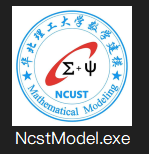
\includegraphics{figure/1.png}
    \caption{软件运行方式}
    \label{fig:exe}
\end{figure}

如图\ref{fig:exe}所示,双击即可运行,免安装。

\subsection{软件更新}

当软件更新到最新版本时,旧版本将无法使用。

\begin{remark}
特意采用了这种开发方式,保证用户使用最新的软件。
\end{remark}

\section{问题反馈}

如果本软件对你造成了困扰,你有两种解决方案,第一种是直接删除,第二种就是来Github进行反馈,
恕不接受QQ或微信反馈问题。邮件反馈也可以,但不利于问题的积累与展示。

\subsection{关于提交}

\begin{itemize}
  \item 对于邮件,详细描述问题即可。即在XX情况下,我点击了XX页面的XX按钮,没有反应、卡死;
  或点击了XX页面的XX按钮却没有按想象中的进行。最好附有截图,拍照恕不回复。
  \item 关于Github,Pull Request 或者 issue 均可,描述问题同上。
\end{itemize}

\begin{remark}
    GitHub是Git的托管服务,Pull Request 或者 issue是Github中常见的软件开方式, 便于开发者进行代码审查和BUG追踪等
    。Git是一种版本管理软件, 建议任何专业的用户掌握基本的Git用法,文件丢失、恢复一个月之前的文件等
    常见问题均可由Git解决。
\end{remark}

\section{协作人员招募}

当然,如果你有兴趣参与软件的后续开发与性能改善,恰好你有不错的编程经验,
并掌握相关的软件开发技术包括但不限于:Git、Qt、Python、Linux和SQL。可以随时联系我,代码放到了网上,到时候我邀请你,相互交流。

但也不仅仅限制与Qt,无论你是Java还是Python,无论是GUI开发还是Web开发,你的想法仍然会受到我们的欢迎。
当然,开发也会有专门的文档记录,这里是使用文档。

也许你不会编程,但仍然想为本软件尽一分力,欢迎把这份文档翻译为英文(不限于此),在此感谢你无私的奉献!

\section{捐赠与致谢}

捐赠就不必了,大学四年一晃而过,劝君珍惜少年时。无论建模与否,也许是电子设计,也许是ACM程序设计,做好自己的选择,
热爱与认真对待自己的选择就是对我们和对你自己而言最好的捐赠。

也致谢那些年建模遇到的所有小伙伴和老师们,此去经年,有缘再见。

\chapter{软件使用}

\section{确认身份}

如图\ref{fig:verify}所示,确认身份界面中有两个选项,分别为管理员身份和游客身份。管理员身份能进行信息的管理,如录入教师信息、比赛信息和学院专业信息等;而游客身份只能查阅信息,假设你暗恋某人,你可以输入他的学号或姓名(重名时不能保证唯一)对他的获奖情况进行查询。当然,也能查询到你情敌成功参赛的信息。
\begin{figure}[h]
    \centering
    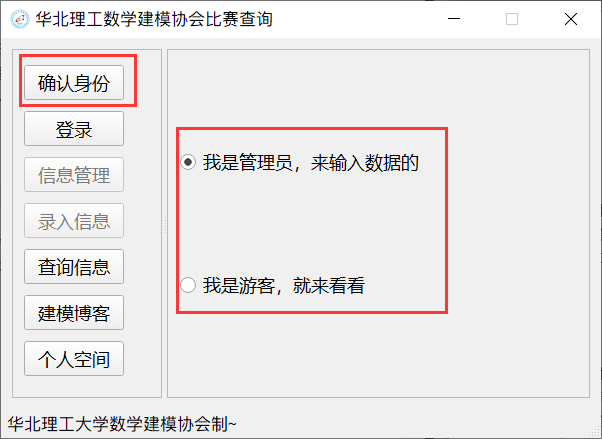
\includegraphics[width=10.5cm, height=8cm]{figure/2.png}
    \caption{确认身份界面}
    \label{fig:verify}
\end{figure}

\begin{remark}
管理员权限只对建模协会内部的管理人员开放。
\end{remark}

\section{登陆界面}

恰好此时的你是管理员,那么输入建模协会提供给你的帐号密码,点击确认按钮且帐号密码没有错误,此时的你就能登录,
如图\ref{fig:login}。当然,你也可以滥用职权随意录入信息,反正这里的信息仅供参考,学院加分又不认这个。

\begin{figure}[h]
    \centering
    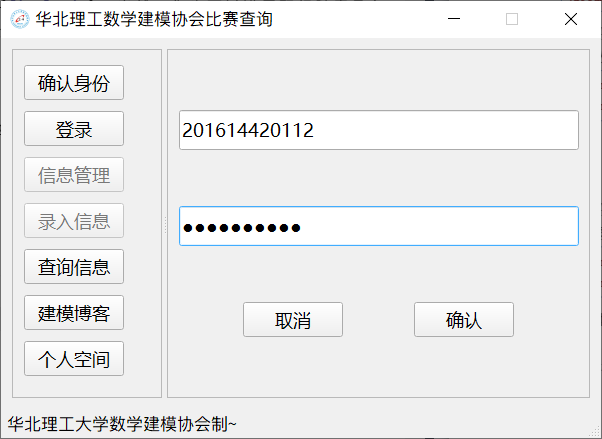
\includegraphics[width=10.5cm, height=8cm]{figure/3.png}
    \caption{确认身份界面}
    \label{fig:login}
\end{figure}

\begin{remark}
密码已加密,也做了注入攻击的防护措施。
\end{remark}

\begin{remark}
切换登录账号时,请退出软件并重新登录。
\end{remark}

\newpage

如果你是超级管理员,你将解锁全部功能,如图\ref{fig:superadmin}。

\begin{figure}[h]
    \centering
    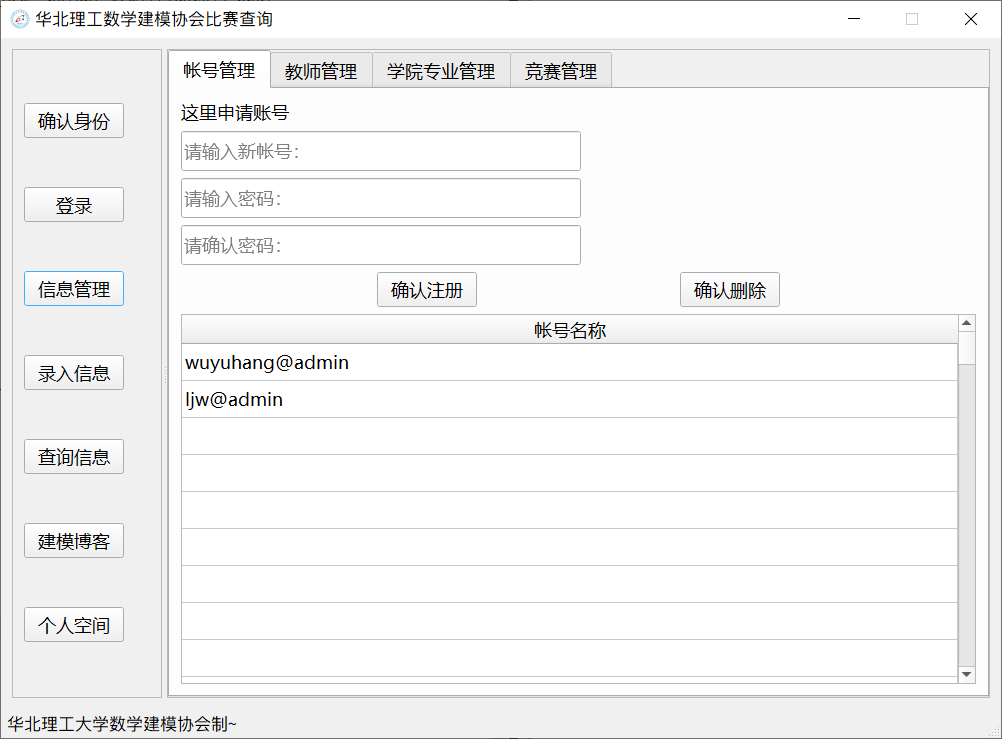
\includegraphics[width=10.5cm, height=8cm]{figure/4.png}
    \caption{超级管理员界面}
    \label{fig:superadmin}
\end{figure}

\newpage

如果你只是普通管理员,将解锁录入信息的功能,如图\ref{fig:admin}。

\begin{figure}[h]
    \centering
    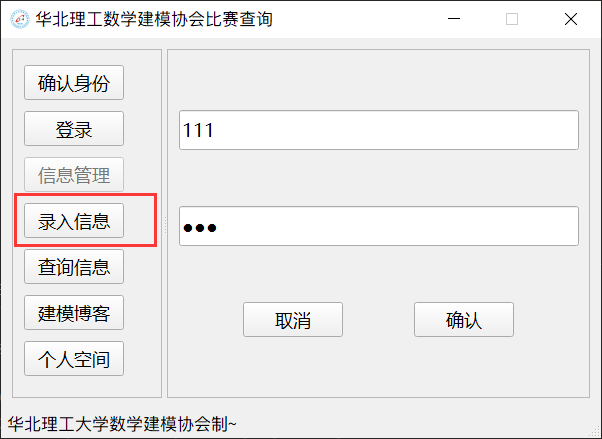
\includegraphics[width=10.5cm, height=8cm]{figure/5.png}
    \caption{普通管理员界面}
    \label{fig:admin}
\end{figure}

\section{查询信息}

任何用户均能自由使用查询信息的功能, 无论是查找心仪教师的带队信息, 还是具体到某一个人的参赛信息, 
整体界面如\ref{fig:query}所示。

\begin{figure}[h]
    \centering
    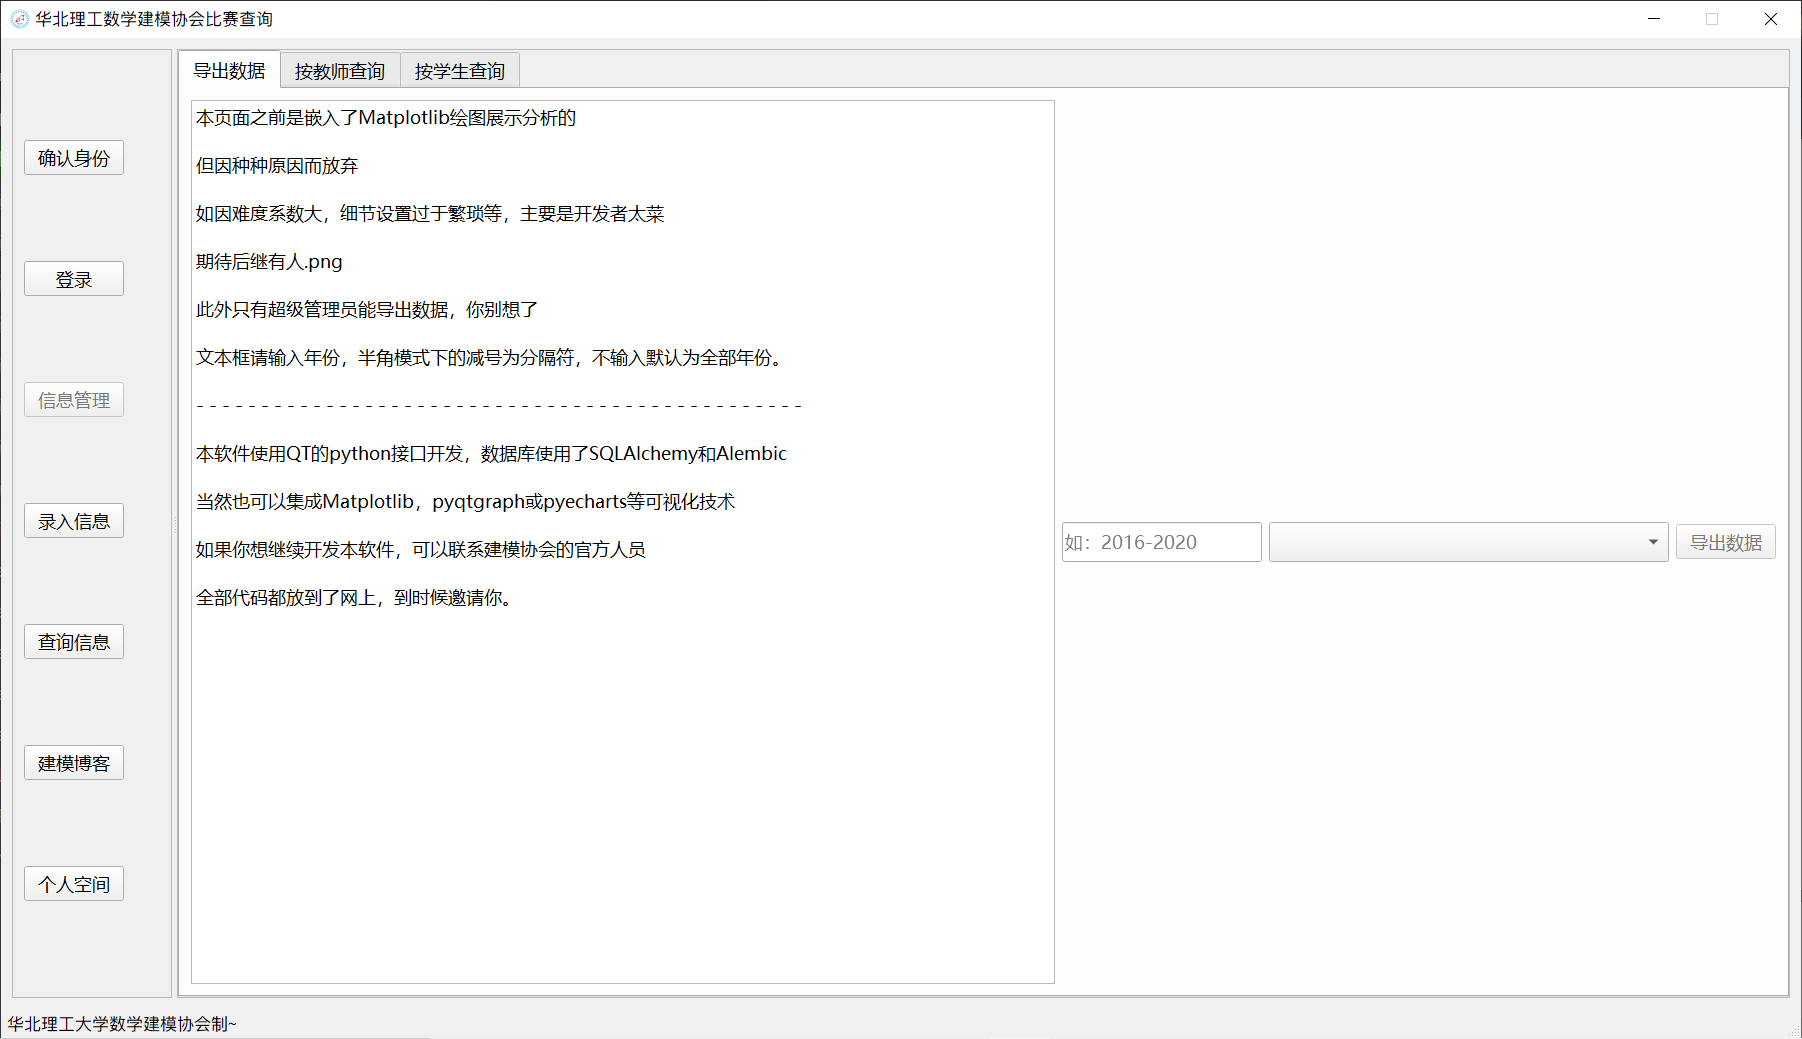
\includegraphics[width=11cm, height=7cm]{figure/6.png}
    \caption{查询信息界面}
    \label{fig:query}
\end{figure}

在按教师查询中,通过下拉列表,点击对应的指导教师即可查询对应老师带领队伍的获奖信息,如图\ref{fig:query_teacher}。

\begin{figure}[h]
    \centering
    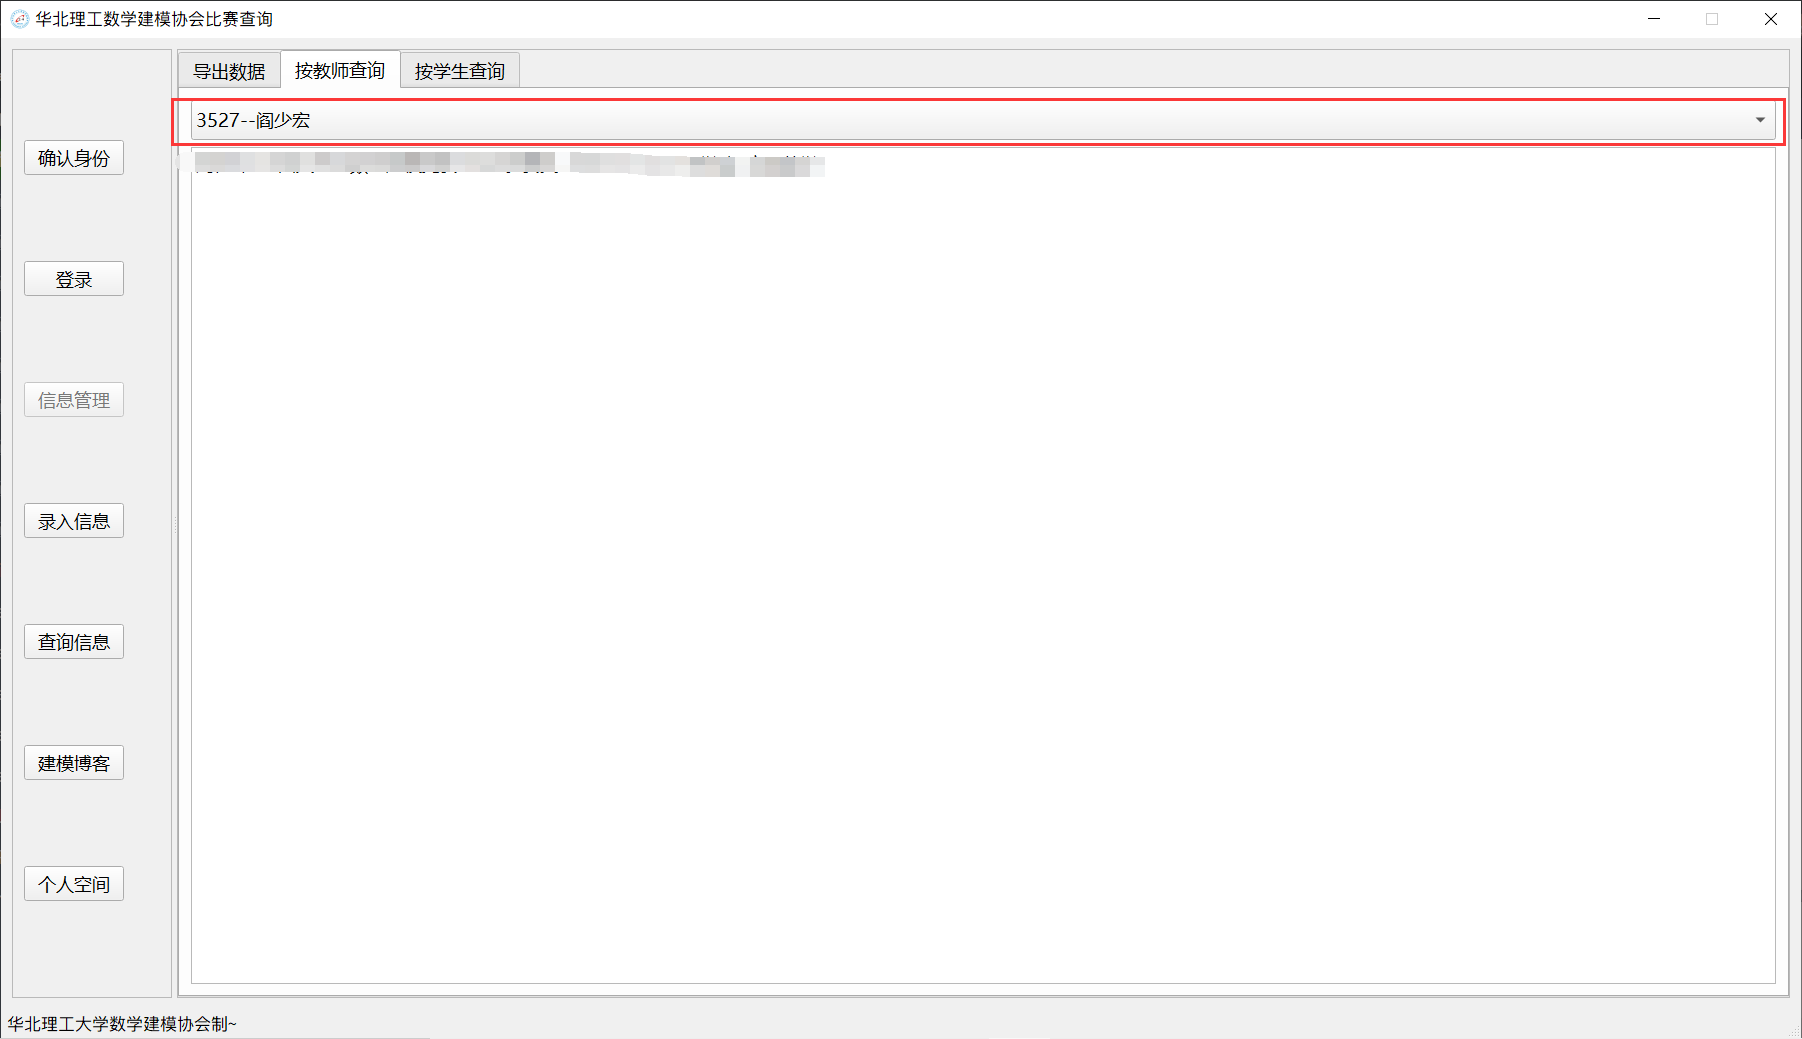
\includegraphics[width=11cm, height=8cm]{figure/7.png}
    \caption{查询教师信息}
    \label{fig:query_teacher}
\end{figure}

\newpage

在按学生查询中,输入学生的姓名或学号,回车即可查询,如图\ref{fig:query_student}。当然现在还查询不了, 信息尚未录入。

\begin{figure}[h]
    \centering
    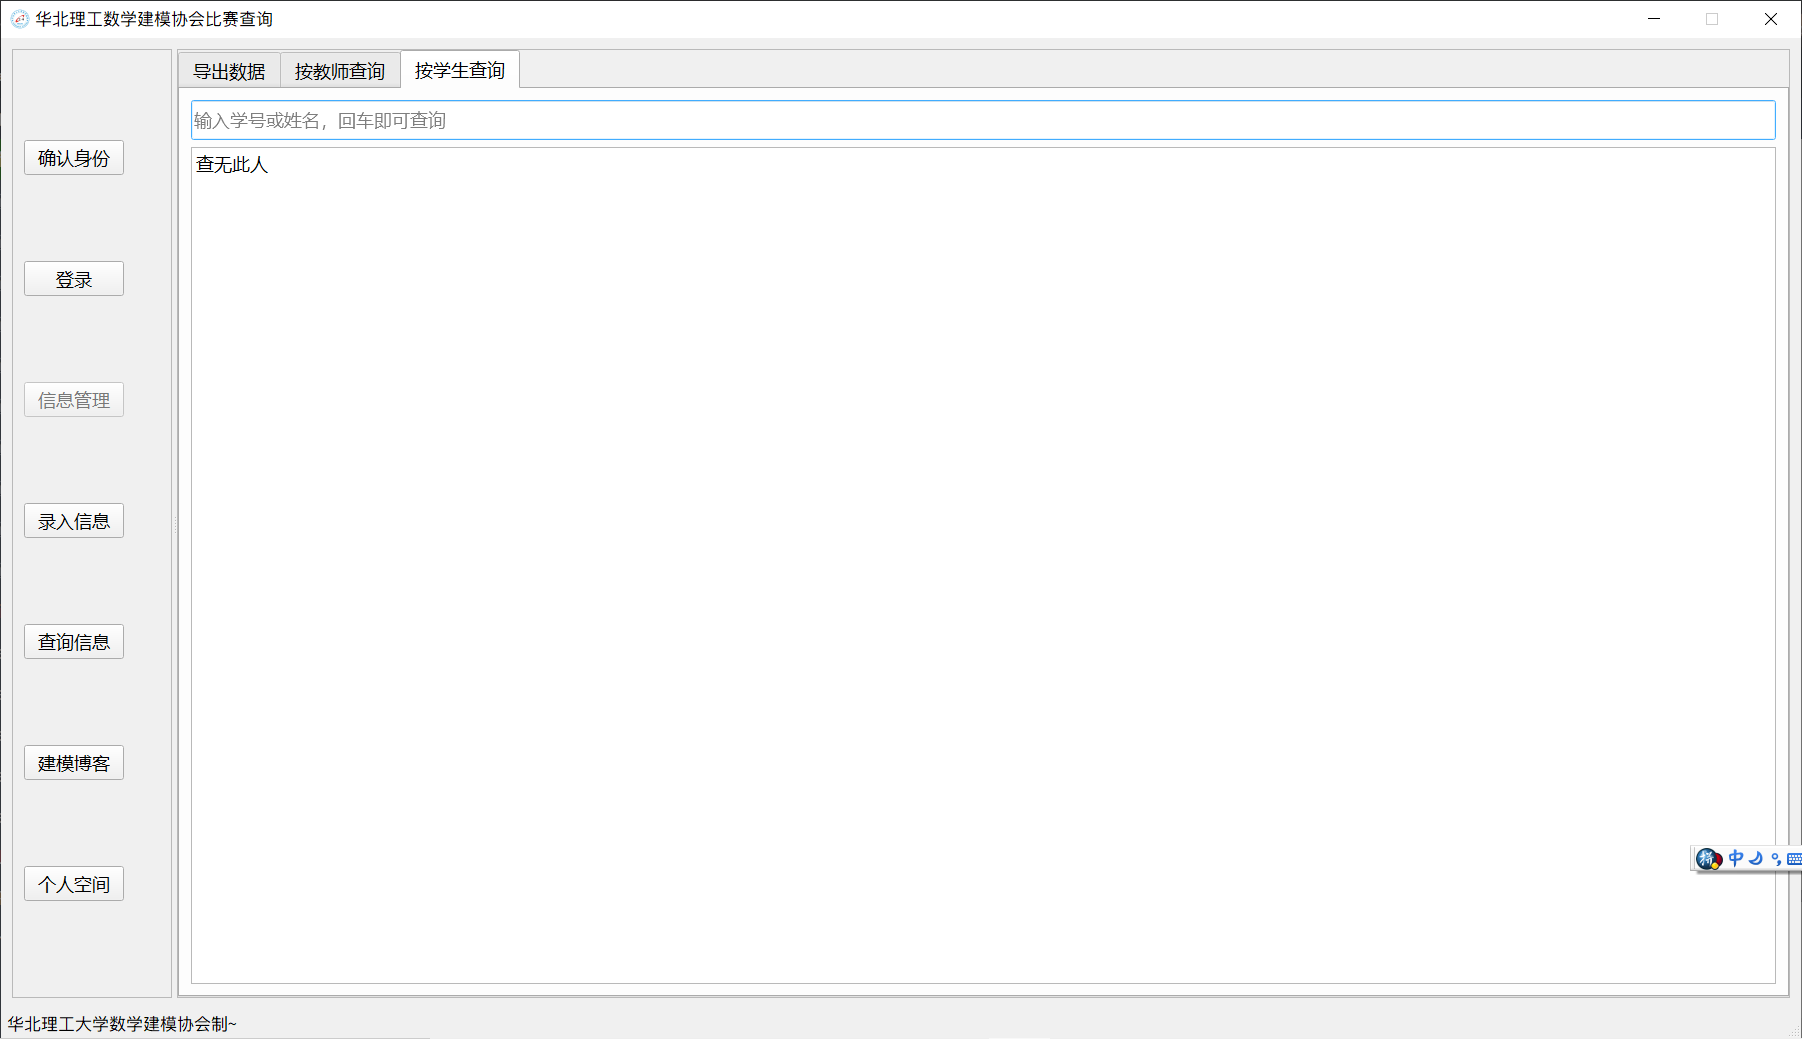
\includegraphics[width=12cm, height=8cm]{figure/8.png}
    \caption{查询学生参赛信息}
    \label{fig:query_student}
\end{figure}

导出数据仅超级管理员可用,输入年份起止,不支持输入月份。
通过下拉列表选择比赛或全部比赛,即可导出excel格式的数据,如图\ref{fig:export_data}。

\begin{figure}[h]
    \centering
    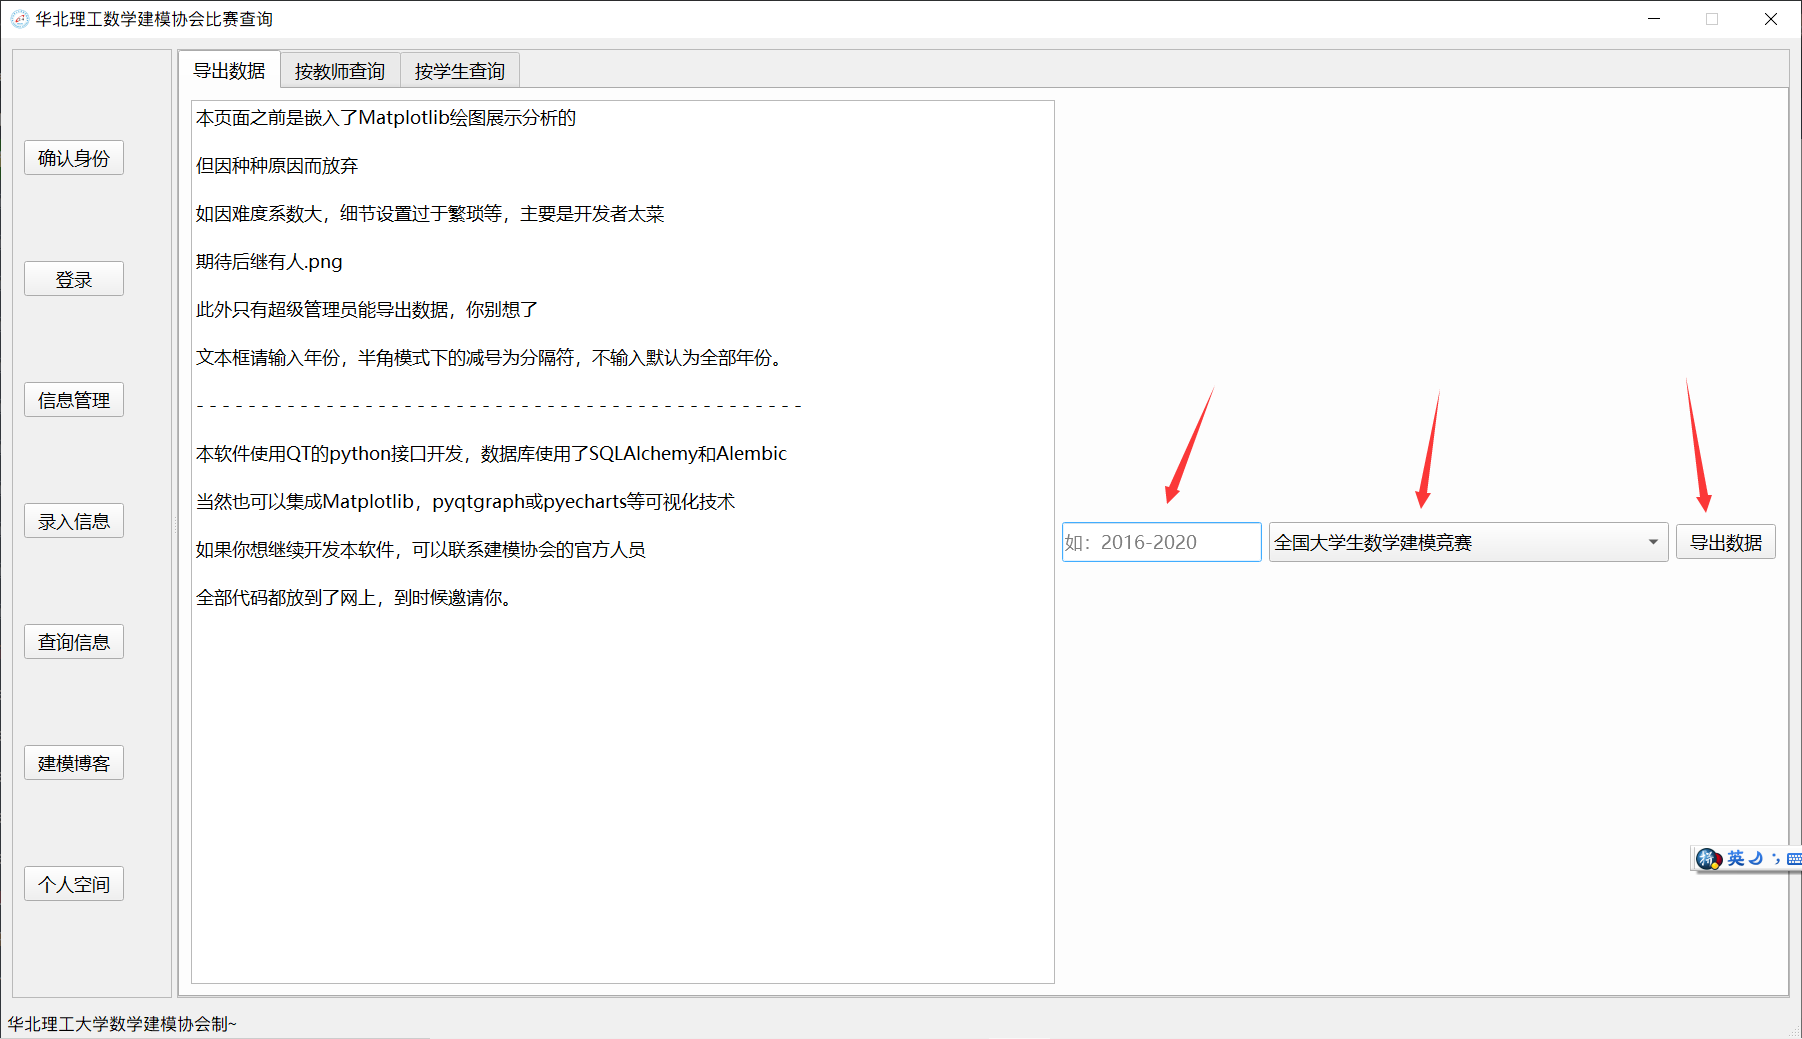
\includegraphics[width=12cm, height=8cm]{figure/9.png}
    \caption{导出参赛数据}
    \label{fig:export_data}
\end{figure}

\newpage

\section{建模博客}

在此导入建模学子的博客,展示建模学子的风采。当然,不会插入借助第三方搭建的博客,如CSDN,知乎等,
文章质量良莠不齐,且有广告插入。点击对应的人员即可调用系统浏览器打开博客,如图\ref{fig:blog}。

\begin{figure}[h]
    \centering
    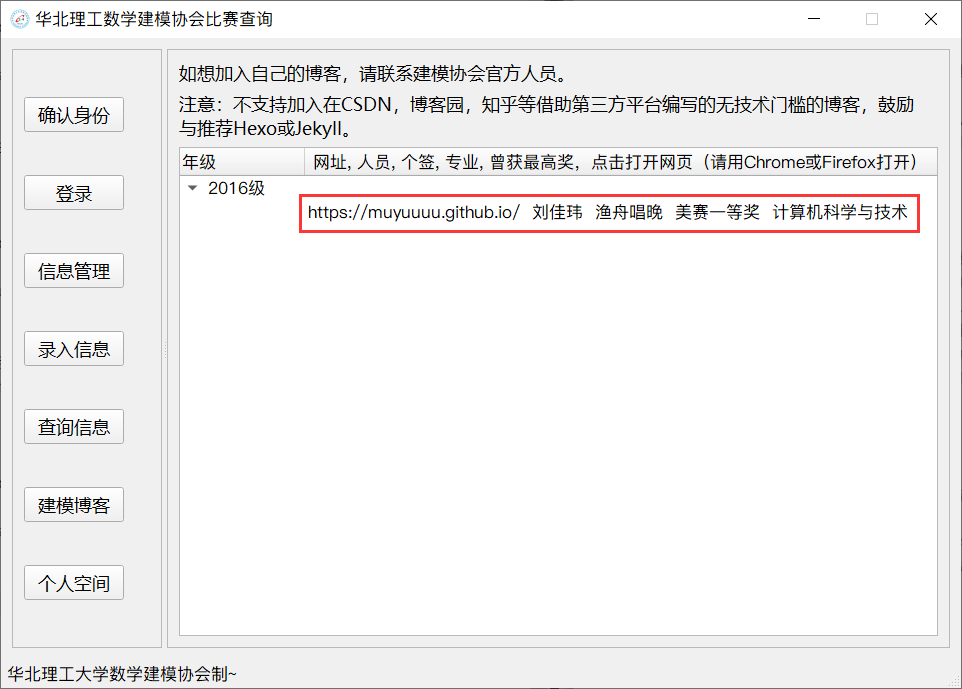
\includegraphics[width=10cm, height=8cm]{figure/10.png}
    \caption{博客展示区}
    \label{fig:blog}
\end{figure}

\section{个人空间}

预留的接口,设计目的是让建模学子展示自己,照片、个签或参赛经历等,方便找队友,找对象(误)等,但尚未开发,
主要是开发人员不会Web开发, 如图\ref{fig:space}。

\begin{figure}[h]
    \centering
    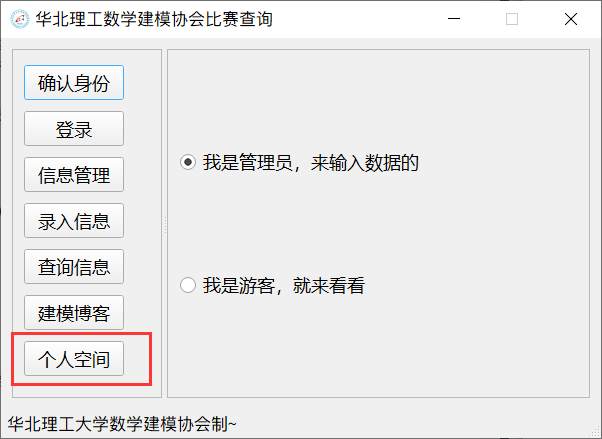
\includegraphics[width=10.5cm, height=8cm]{figure/11.png}
    \caption{个人空间}
    \label{fig:space}
\end{figure}

\chapter{结语}

经不断反馈BUG与调试,也在不断的修正和完善软件。截至此次更新,Github共有40次左右的提交,正式版本有2次,最后祝各位愉快度过建模生涯。

\datechange{2020/05/10}{版本 2.0 正式发布}

\begin{change}
  \item 1.0 为内部测试版本。
  \item 2.0 修正管理员登录的身份验证紊乱BUG。
  \item 重新定制软件尺寸和控件尺寸,适应高分屏电脑。
  \item 修改专业同名无法录入的情况,如以升学院的电气工程和电气学院的电气工程。
\end{change}

\end{document}
